\documentclass{article}
\usepackage[utf8]{inputenc}
\usepackage{physics}
\usepackage{amsmath}
\usepackage{showlabels}
\usepackage{amssymb}
\usepackage{natbib}
\usepackage{graphicx}
\usepackage{array}

\renewcommand{\vec}[1]{\ensuremath{\mathbf{#1}}}
\newcommand{\uvec}[1]{\ensuremath{\hat{\mathbf{#1}}}}
\newcommand{\figurewidth}{0.4\textwidth}
\newcommand{\widefigurewidth}{0.8\textwidth}

% One should follow the following naming scheme:
% HW1_SHI_JIALE.zip

\title{Machine Learning\\[1em] Homework 1}
\author{Jiale Shi}
%\date{Dec/10/2018}
\begin{document}
\maketitle

\newpage
\section{Beta Updating from censored likelihood and MLE for uniform distribution}
\textbf{A} Suppose we toss a coin $n=5$ times. Let $X$ be the number of heads. Assume that we observe that there are fewer than 3 heads, however, we don't known the exact number. We consider the prior probability of heads to be $p(\theta) = \rm Beta(\theta|1,1)$. Compute the posterior $p(\theta|X<3)$ up to normalization constant (i.e., derive expression proportional to $p(\theta|X<3)$).
\\
\textbf{Solution:} \\
Since the prior probability of heads is $p(\theta) = \rm Beta(\theta|1,1)$, it is equal to uniform distribution and independent with $\theta$.

\begin{equation}
\begin{aligned}
p(\theta|X<3) & \propto p(X<3|\theta)p(\theta) \\
& \propto p(X<3|\theta)\\
& = p(X=0|\theta)p(\theta) + p(X=1|\theta)p(\theta) + p(X=2|\theta)p(\theta) \\
& = 1\cdot \theta^{0}(1-\theta)^{5}+ 5 \cdot \theta^{1}(1-\theta)^{4} + 10 \cdot \theta^{2}(1-\theta)^{3} \\
& = \rm Bin(0|\theta,5)+Bin(1|\theta,5)+Bin(2|\theta,5)
\end{aligned}
\end{equation}
\\
\textbf{B} Consider a uniform distribution centred on 0 with width $2a$. The density function is given as 
\begin{equation}
    p(x) = \frac{1}{2a} \mathbb{I}(x \in [-a,a])
\end{equation}
\\
(a) Given a dataset $x_1,...,x_n$,what is the MLE of $a$? \\
\textbf{Solution:} \\
\begin{equation}
\begin{aligned}
& p(D|a) = \left[\frac{1}{\rm size(\textit{a})}\right]^{n} = \left[\frac{1}{ 2a}\right]^{n}  \\
& \hat{a}^{mle} = {\rm argmax} p(D|a) = \max {\rm abs}(x_1,...,x_n)
\end{aligned}
\end{equation}
The MLE of $a$ is the maximum absolute value of the given data set $x_1,...,x_n$.
\\
(b) What probability would the model assign to $\hat{x}_{n+1}$ using the MLE estimate of $a$?\\
\textbf{Solution:} \\
\begin{equation}
    p(\hat{x}_{n+1}|\hat{a}^{mle}) = \left\{ \begin{array}{rcl}
         \frac{1}{2\hat{a}^{mle}} & \mbox{for}
         & \abs{\hat{x}_{n+1}} \leq \hat{a}^{mle} \\ 
         0  & \mbox{for} & \abs{\hat{x}_{n+1}} > \hat{a}^{mle} 
         \end{array} \right\}
\end{equation}
\\
(c)Do you see any problem with the above approach? If yes, briefly suggest a better alternative. \\
\textbf{Solution:} \\
In (b),
\begin{equation}
\begin{aligned}
    p(\hat{x}_{n+1}|\hat{a}^{mle}) & =  0  & \mbox{for} & \abs{\hat{x}_{n+1}} > \hat{a}^{mle} 
\end{aligned}
\end{equation}
Therefore, using MLE can perform quite poorly when the sample data set size is small. This is called the \textbf{zero count problem} or the \textbf{sparse data problem}, and frequently occurs when estimating counts from small amounts of data. A better alternative would be calculate the posterior by using Bayesian analysis and choosing a suitable prior. 

\newpage
\section{Bayesian analysis for Uniform distribution and the Taxicab problem}
\textbf{A} Consider the uniform distribution $\mathcal{U}(0,\theta)$. Given the Pareto prior, the joint distribution of $\theta$ and $\mathcal{D} = (x_1,...,x_{N})$ is
\begin{equation}
p(\mathcal{D},\theta) = \frac{Kb^{K}}{\theta^{N+K+1}} \mathbb{I}(\theta \geq \max(\mathcal{D}))   
\end{equation}
Let $m = \max(\mathcal{D})$. The evidence (the probability that all $N$ samples came from the same uniform distribution) is
\begin{equation}
\begin{aligned}
p(\mathcal{D}) & = \int_{m}^{\infty} \frac{Kb^{K}}{\theta^{N+K+1}} d\theta \\
& = \left\{ \begin{array}{rcl}
         \frac{K}{(N+K)b^{N}} & \mbox{if }
         &  m \leq b\\ 
         \frac{Kb^{K}}{(N+K)m^{N+K}}  & \mbox{if}  & m>b  
         \end{array} \right\}
\end{aligned} 
\end{equation}
Derive the posterior $p(\theta | \mathcal{D})$ and show that it can be expressed as a Pareto distribution.
\\
\textbf{Solution:}
\begin{equation}
  p(\theta | \mathcal{D}) = \frac{p(\mathcal{D},\theta)}{p(\mathcal{D})} = \frac{Kb^{K}}{\theta^{N+K+1}} \mathbb{I}(\theta \geq \max(\mathcal{D},b))   \frac{1}{p(\mathcal{D})} 
\end{equation}
\\
The first case, if $m \leq b$,
\begin{equation}
\begin{aligned}
 p(\theta | \mathcal{D}) & = \frac{Kb^{K}}{\theta^{N+K+1}} \mathbb{I}(\theta \geq \max(\mathcal{D},b))  \frac{(N+K)b^{N}}{K} \\
 & = \frac{(N+K)b^{N+K}}{\theta^{N+K+1}} \mathbb{I}(\theta \geq b)) \\
 & = Pareto(\theta|N+K,b)
\end{aligned}
\end{equation}

The second case, if $m > b$,
\begin{equation}
\begin{aligned}
 p(\theta | \mathcal{D}) & = \frac{Kb^{K}}{\theta^{N+K+1}} \mathbb{I}(\theta \geq \max(\mathcal{D},b))  \frac{Kb^{K}}{(N+K)m^{N+K}} \\
 & = \frac{(N+K)m^{N+K}}{\theta^{N+K+1}} \mathbb{I}(\theta \geq m)) \\
 & = Pareto(\theta|N+K,m)
\end{aligned}
\end{equation}

Therefore, 
\begin{equation}
  p(\theta | \mathcal{D}) = Pareto(\theta|N+K,\max(m,b))  
\end{equation}
\\
\textbf{B} Suppose you arrive in a new city and see a taxi numbered 100. How many taxis are there in this city? Let us assume taxis are numbered sequentially as integers starting from 0, up to some unknown upper bound $\theta$. Hence the likelihood function is $p(x) = \mathcal{U}(0,\theta)$.
\\
(a) Suppose we see one taxi numbered 100. Using an non-informative prior on $\theta$ of the form $p(\theta) = \rm Pa(\theta|0,0) \propto \frac{1}{\theta}$. What is the posterior $p(\theta | \mathcal{D})$?
\\
\textbf{Solution:}\\
$p(\theta) = \rm Pa(\theta|0,0) \propto \frac{1}{\theta}$, therefore, $b=0$, $K=0$. \\
Suppose we see one taxi numbered 100, therefore, $\mathcal{D}={100}$, $m=100$, $N=1$.
Using the Bayesian analysis result from Part. A.
\begin{equation}
\begin{aligned}
  p(\theta | \mathcal{D}) & = Pareto(\theta|N+K,\max{(m,b)})  \\
  & =  Pareto(\theta|1+0,\max(100,0)) \\
  & =  Pareto(\theta|1,100)
\end{aligned}
\end{equation}
\\
(b) Compute the posterior mean, mode and median number of taxis in the city, if such quantities exist. \\
\textbf{Solution:}\\
From wikipedia, \\
The posterior mean of  $Pareto(\theta|\alpha,x_{m})$ is equal to $E[\theta|D] = \frac{\alpha x_{m}}{\alpha -1}, \alpha>1$. But in this Pareto distribution,$Pareto(\theta|1,100)$, $\alpha=1$ and $x_{m}=100$. Therefore, the posterior mean does not exist. \\
The mode of this Pareto distribution, ${\rm mode}(\theta|D) = x_{m} = 100$ \\
The median of this Pareto distribution, ${\rm median}(\theta|D) = x_{m} (2)^{\frac{1}{\alpha}} = 100 (2)^{1} = 200$
\\
(c) Rather than trying to compute a point estimate of the the number of taxis, we can compute the predictive density over the next taxicab number using
\begin{equation}
    p(D^{'}|\mathcal{D},\alpha) = \int p(D^{'}|\theta) p(\theta|\mathcal{D},\alpha) d\theta = p(D^{'}|\beta)
\end{equation}
where $\alpha = (b,K)$ are the hyperparameters and $\beta = (c,N+K)$ are the updated hyperparameters. Now consider the case $\mathcal{D} = \{m\}$, and $D^{'} = \{x\}$. Using Part A of this problem, write down the expression for $p(x|\mathcal{D},\alpha)$. As above, consider, $b=K=0$. \\
\textbf{Solution:} \\
In order to compute the predictive density over the next taxicab number $m$, we need to calculate the posterior $p(\theta|\mathcal{D})$ with $N=1$,$b=K=0$
\begin{equation}
\begin{aligned}
p(\theta|\mathcal{D}) & = Pareto(\theta|N+K,\max{(m,b)}) \\
& = Pareto(\theta|1+0,\max{(m,0)}) \\
& = Pareto(\theta|1,m)
\end{aligned}
\end{equation}
We can use this posterior on $\mathcal{D}$ as a "prior" for the inference on the next taxicab $D^{'}$.
This new "prior" for the next taxicab $p(\theta) = Pareto(\theta,K^{'}=1,b^{'}=m)$.$N^{'} = 1$ and $m^{'} = \max{(D^{'})} = x$.

Using equation from part A.
\begin{equation}
\begin{aligned}
p(x|\mathcal{D},\alpha) & = \frac{K^{'}}{(N^{'}+K^{'}) {b^{'}}^{N^{'}}} \mathbb{I} (m^{'} \leq b^{'}) + \frac{K^{'}{b^{'}}^{K^{'}}}{(N^{'}+K^{'}){m^{'}}^{N^{'}+K^{'}}} \mathbb{I} (m^{'} > b^{'}) \\
& = \frac{1}{2m} \mathbb{I} (x \leq m) + \frac{m}{2x^2} \mathbb{I} (x > m)
\end{aligned}
\end{equation}
\\
(d) Use the predictive density formula to compute the probability  that the next taxi you will see (say, the next day) has the number 100, 50 or 150. \\
\textbf{Solution:} \\
\begin{equation}
\begin{aligned}
& p(x= 100|\mathcal{D},\alpha)   = \frac{1}{2m} \mathbb{I} (100 \leq m) + \frac{m}{20000} \mathbb{I} (100 > m) \\
& p(x= 50|\mathcal{D},\alpha)   = \frac{1}{2m} \mathbb{I} (50 \leq m) + \frac{m}{5000} \mathbb{I} (50 > m) \\
& p(x= 150|\mathcal{D},\alpha)  = \frac{1}{2m} \mathbb{I} (150 \leq m) + \frac{m}{45000} \mathbb{I} (150 > m) 
\end{aligned}
\end{equation}
\\
(e) Briefly describe (1-2 sentences) some ways you might make the model more accurate at prediction. \\
\textbf{Solution:} \\
(1) Use an informative prior on $\theta$ instead of non-informative prior.\\
(2) Use a discrete probability distribution since $m$ and $b$ are discrete integer in this problem. In addition, instead of using integral, use summation.

\newpage
\section{Naive Bayes}
\subsection{}
Consider a Naive Bayes model (multivariate Bernouli version) for spam classification with the vocabulary $V=$"secret", "offer", "low",  "price", "valued", "customer", "today", "dollar", "million", "sports",  "is", "for", "play", "healthy", "pizza". We have the following example, spam messages "million dollar offer", "secret offer today","secret is secret" and normal messages, "low price for valued customer","play secret sports today","sports is healthy","low price pizza". Given the MLEs for the following parameters: $\theta_{\rm spam}$, $\theta_{\rm secret | \rm spam}$, $\theta_{\rm secret | \rm non-spam}$, $\theta_{\rm sports | \rm non-spam}$, $\theta_{\rm dollar | \rm spam}$.
\\
\textbf{Solution:}
MLE
\begin{equation}
    \hat{\theta}_{k}^{mle} = \frac{N_{k}}{N}
\end{equation}

\begin{equation}
\begin{aligned}
& N_{\rm spam} = 3 \\
& N_{\rm non-spam} = 4 \\
& N_{\rm secret,\rm spam} = 2 \\
& N_{\rm secret, \rm non-spam} = 1 \\
& N_{\rm sports, \rm non-spam} = 2 \\
& N_{\rm dollar | \rm spam} = 1
\end{aligned}
\end{equation}

\begin{equation}
\begin{aligned}
& \theta_{\rm spam} = \frac{3}{3+4} = \frac{3}{7} \\
&\theta_{\rm secret | \rm spam} = \frac{2}{3} \\
&\theta_{\rm secret | \rm non-spam} = \frac{1}{4} \\
&\theta_{\rm sports | \rm non-spam}=\frac{2}{4} = \frac{1}{2}\\
&\theta_{\rm dollar | \rm spam} = \frac{1}{3} 
\end{aligned}
\end{equation}
\\
\subsection{}
Write a code for a Naive Bayes classifier (both training and prediction) and use it for the two data sets provided at this link. Both the data sets have four variables namely, $\rm Xtrain$, $\rm Xtest$, $\rm ytrain$ and $\rm ytest$. Train the Naive Bayes classifier based on $\rm Xtrain$ and $\rm ytrain$ and test it based on $\rm Xtest$ and $\rm ytest$. Report the misclassification rate for both the data sets.\\
\textbf{Solution:} \\
For first dataset "Problem3b1.mat", there are 4 classes. Misclassification rate on train is 18.92\%, on test is 19.3\%.
\\
For second dataset "Problem3b2.mat", there are 2 classes. Misclassification rate on train is 8.33\%, on test is 18.67\%.

\newpage
\section{Emperical Bayes}
Consider the problem of predicting cancer rates in various cities. In particular, suppose we measure the number of people in various cities, $N_{i}$, and the number of people who died of cancer in those cities, $x_{i}$. We assume $x_{i} \sim \rm Bin(N_{i}, \theta_{i})$, and we want to estimate the cancer rates $\theta_{i}$. One way is to estimate the parameters separately, but this will inevitably suffer from the sparse data problem. On the other hand, parameter trying for this problem will be too strong an assumption. A compromise is to assume that the parameters $\theta_{i}$ are similar but there may be city-specific variations. This can be modelled by assuming that the $\theta_{i}$ are drawn from some common distribution. Assuming that $\theta_{i} \sim \rm Bin(a, b)$, the joint distribution can be written as:
\begin{equation}
    p(\mathcal{D},\theta,\eta|N) = p(\eta) \prod_{i=1}^{N} \rm Bin(x_{i}|\theta_{i},N_{i}) Beta(\theta_{i}|\eta)
\end{equation}
where $\eta = (a,b)$. With this set up, the problem can be solved using two methods. In the first method, we can adopt a fully Bayesian approach by assigning an appropriate prior. However, with this setup, we will have to resort to some sampling based approach which will be covered later in the course. The other method is to estimate point estimates for $\eta$ by using $\mathcal{D}$. This method is known as the Empirical Bayes. Note that this method violates the basic assumption of Bayesian statistics as the prior depends on the data.

Write a computer code for estimating the parameters, $\theta_{i}$ by using empirical Bayes. For estimating the parameters $\eta$ is empirical Bayes, you can utilize the fixed point method proposed by Minka. The MATLAB code for the fixed point method and the cancer data set can be found at this link. The data set has a structure data which, in turn, has two variables $y$ (No. of persons with cancer) and $n$ (Total population of the city). \\
\textbf{Solution:} \\
We use Empirical Bayes to deal with this problem. The reasons why we use Empirical Bayes have been partially stated in the problem. I would state again: if we estimate them separately, this would suffer from the sparse data problem (underestimation of the rate of cancer due to small $N_i$); if we assume all the $\theta_{i}$ are the same, this is called parameter tying, and this assumption that all the cities have the same rate is a rather strong one. A compromise approach is to assume that the $\theta_{i}$ are similar, but that there may be city-specific variations. The data-poor cities borrow statistical strength from the data-rich city.\\
Note that it is important that we get $\eta=(a,b)$ from the data. If we just assume it to be constant, the $\theta_{i}$ will be conditionally independent for all the cities, and there will be no information flow between them. By contrast, by treating $\eta=(a,b)$ as unknown (hidden variable), we allow  the data-poor cities to borrow statistical strength from the data-rich ones.\\
If we just use MLE (in third row of Figure 1), we would find that the MLE of  city 20 is 0 since city 20 has a very smaller population. However, it is not reliable because this would suffer from the sparse data problem.
We compute the joint posterior $p(\eta,\theta|\mathcal{D})$. From this we can get the posterior marginals $p(\theta_{i}|\mathcal{D})$ and posterior means $\mathbb{E}(a/a+b|\mathcal{D})$ (in fourth row of Figure 1). The posterior mean is shrunk towards the pooled estimate more strongly for cities with small sample sizes, like city 20. If we use posterior mean, its rate is shrunk more towards to the pop mean. Even for city 10 and 19, their posterior mean are also shrunk towards to the pop mean.

Figure 2 shows the 95\% posterior credible intervals for $\theta_{i}$ for all cities. City 15 has a very large population and has small posterior uncertainty. This data has the largest impact on the posterior estimate of $\eta$, which would in turn influence the estimate of the cancer rates for other cities. 

Figure 1 and Figure 2 are created by using the matlab code offered and adding some modifications. The analyse is based on Zabaras's lectures and Murphy's book \textit{Machine Learning}.

\begin{figure}[h!]
\centering
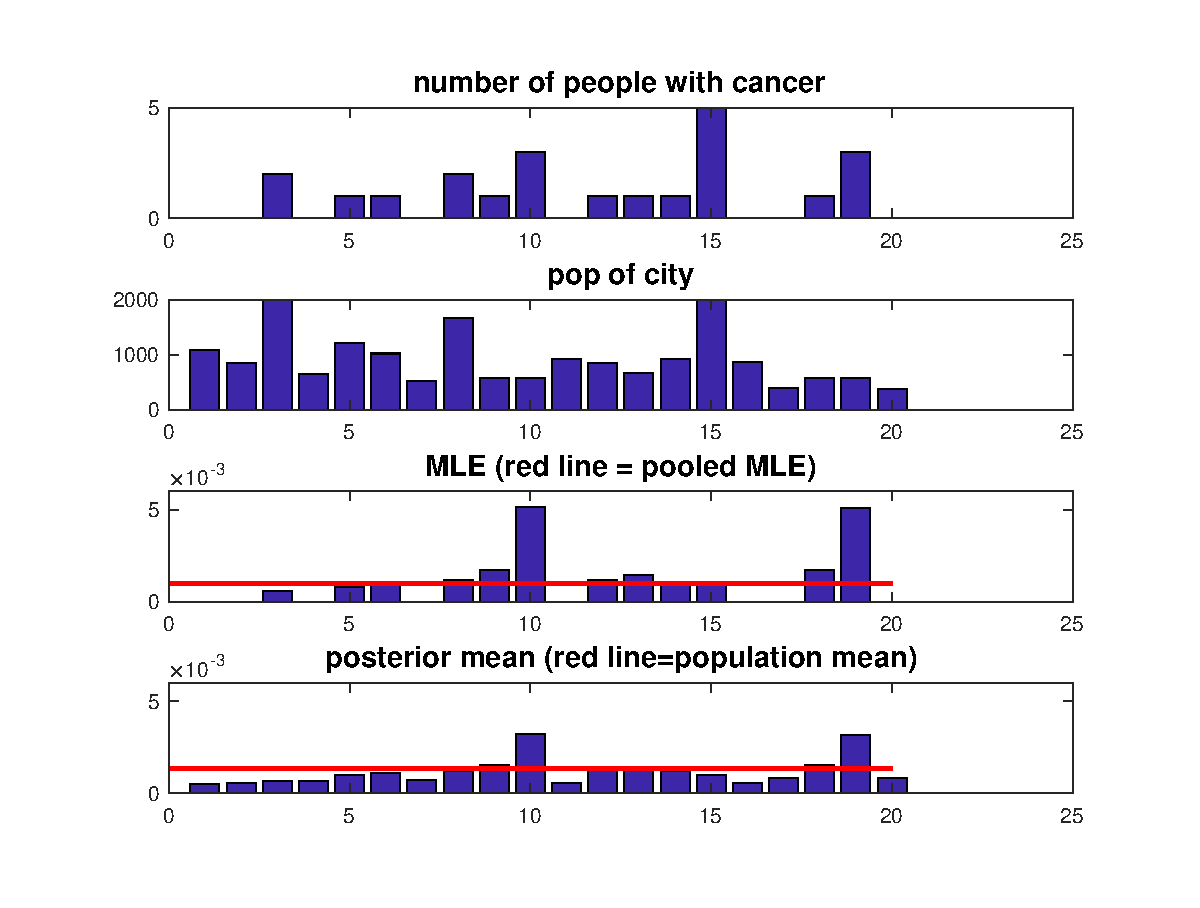
\includegraphics[width=\widefigurewidth]{fig/HW1P4a.eps}
\caption{Results of fitting the model}
%\label{fig:universe}
\end{figure}

\begin{figure}[h!]
\centering
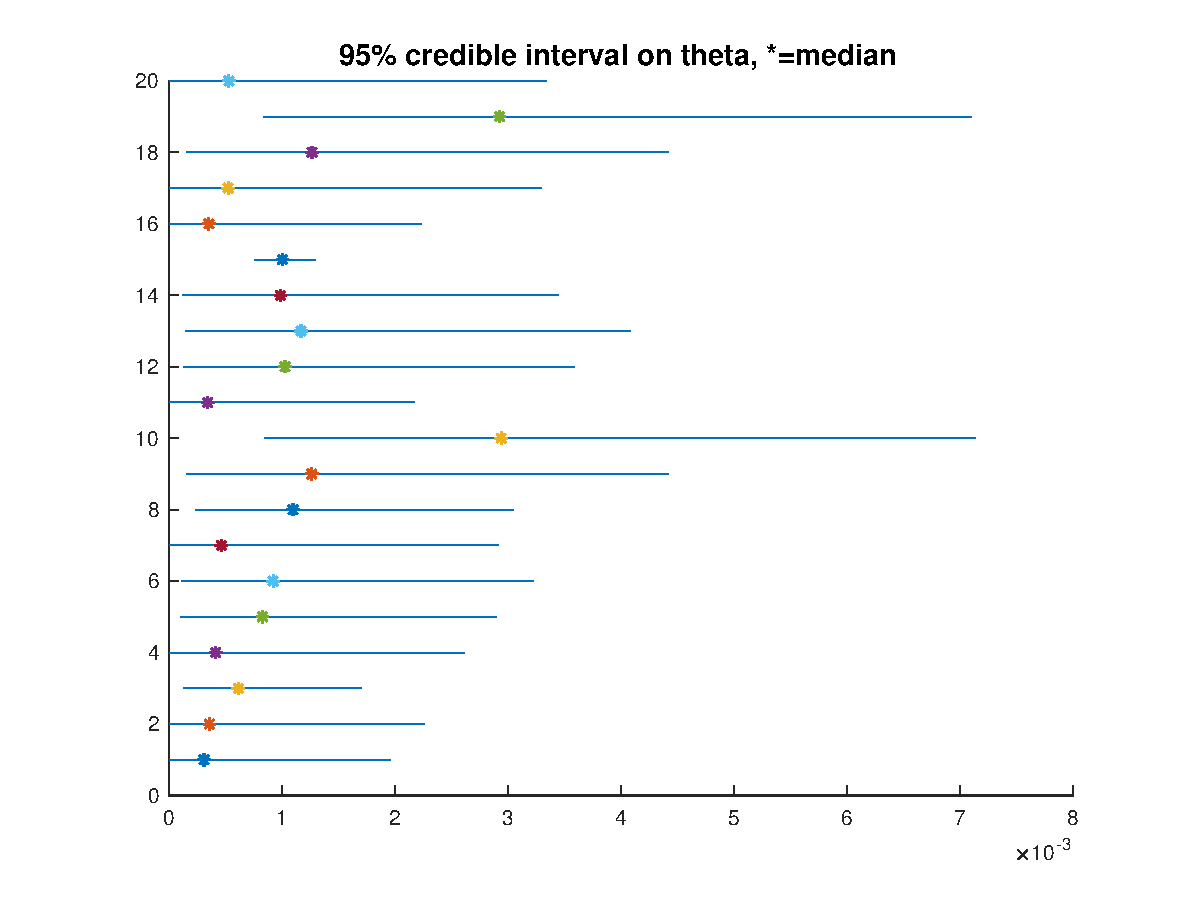
\includegraphics[width=\widefigurewidth]{fig/HW1P4b.eps}
\caption{Posterior 95\% credible intervals on the cancer rates.}
%\label{fig:universe}
\end{figure}

\newpage
\section{Reject option in classifiers and Newsvendor problem}
\textbf{A} In many classification problems one has the option either of assigning $x$ to class $j$ or, if you are too uncertain, of choosing the reject option. If the cost for rejects is less than the cost of falsely classifying the object, it may be the optimal action. Let $\alpha_{i}$ mean you choose action $i$, for $i=,...,C+1$ where  $C$ is the number of classes and $C+1$ is the rejection option. Let $Y = j$ be the true (but unknown) state of nature. We define the loss function as 

\begin{equation}
\begin{aligned}
     \lambda(\alpha_{i}|Y=j) =  \left\{\begin{array}{rcl}
         0 & \mbox{if} & i=j \mbox{and} i,j \in {1,...,C} \\ 
         \lambda_{r}  & \mbox{if} & i=C+1 \\
         \lambda_{s}  & \mbox{otherwise}
         \end{array} \right\}
\end{aligned}
\end{equation}

In other words you incur 0 loss if you correctly classify, you incur $\lambda_{r}$ loss if you choose the reject option and you incur $\lambda_s$ loss if you make a substitution error (misclassification).
\\
(a) Show that the minimum risk is obtained at $Y=j$ if
\begin{equation}
    p(Y=j|x) \geq p(Y=k|x) \forall k
\end{equation}
and

\begin{equation}
    p(Y=j|x) \geq 1 - \frac{\lambda_r}{\lambda_s}
\end{equation}
otherwise we decide to reject.
\\
\textbf{Solution:}\\
If we choose to assign a class $\alpha_{k} \in (\alpha_1, ...,\alpha_C) \forall k$
\begin{equation}
\begin{aligned}
\rho(a|x) = \sum_{i=1}^{C}p(Y=i|x)L(Y=k,\alpha_k) = \sum_{i \neq k}p(Y=i|x)\lambda_s = (1-p(Y=k|x))\lambda_s
\end{aligned}
\end{equation}
\\
If we choose the reject option.
\begin{equation}
\begin{aligned}
\rho(a|x) = \sum_{i=1}^{C}p(Y=i|x)L(Y=i,\alpha_k) =  \sum_{i=1}^{C}p(Y=i|x)\lambda_r = \lambda_r
\end{aligned}
\end{equation}

The risk of obtaining at $Y=j$ is: $(1-p(Y=j|x))\lambda_s$

If the minimum risk is obtained at $Y=j$. Therefore, the risk of obtaining at $Y=j$ should be smaller than both the risks obtained before.
\begin{equation}
\begin{aligned}
& (1-p(Y=j|x))\lambda_s \leq (1-p(Y=k|x))\lambda_s \\
& p(Y=j|x) \geq p(Y=k|x)
\end{aligned}
\end{equation}

and

\begin{equation}
\begin{aligned}
& (1-p(Y=j|x))\lambda_s \leq \lambda_r \\
& p(Y=j|x) \geq 1 - \frac{\lambda_r}{\lambda_s}
\end{aligned}
\end{equation}
\\
(b) Describe Qualitatively what happens as $\frac{\lambda_r}{\lambda_s}$ is increased from 0 to 1.\\
\textbf{Solution:} \\
If $\frac{\lambda_r}{\lambda_s} = 0$, therefore $\lambda_{r} = 0$ and there is no risk in choose the reject option. Then consider the (a), in order to satisfy that the minimum risk is obtained at $Y=j$, $p(Y=j|x) \geq 1 - \frac{\lambda_r}{\lambda_s} = 1$, therefore, $p(Y=j|x) = 1$. \\
If $\frac{\lambda_r}{\lambda_s} = 1$, $\lambda_r= \lambda_s$. This means that the loss of choosing the reject option and making a substitution error (misclassification) are the same. Then the reject option is no valuable. It is better to choose to assign a class since there are chances to meet the true class.\\
If $0<\frac{\lambda_r}{\lambda_s} <1$, with $\frac{\lambda_r}{\lambda_s}$ increases, choosing a reject option becomes less and less interesting and valuable since the loss of reject option becomes larger and larger and become closer and closer to the loss of misclassification.
\\
\textbf{B} Suppose you are trying to decide how much quantity $Q$ of some product (e.q., newspapers) to buy to maximize your profits. The optimal amount will depend on how much demand $D$ you think there is for your product, as well as its cost to you $C$ and its selling price $P$. Suppose $D$ is known but has pdf $f(D)$ and cdf $F(D)$. We can evaluate the expected profit by considering two cases: if $D>Q$, then we sell all $Q$ items, and make profit $\pi = (P-C)Q$; but if $D<Q$, we only sell $D$ items, at profit $(P-C)D$, but have wasted $C(Q-D)$ on the unsold items. So we expected profit if we by quantity $Q$ is
\begin{equation}
    \mathbb{E}_{\pi} = \int_{Q}^{\infty} (P-C) Q f(D) dD +  \int_{0}^{Q} (P-C) D f(D) dD -\int_{0}^{Q} C(Q-D) f(D) dD
\end{equation}
Show that the optimal quantity $Q^*$ (which maximizes the expected profit) satisfies
\begin{equation}
    F(Q^*) = \frac{P-C}{P}
\end{equation}
\\
\textbf{Solution:} \\
\begin{equation}
\begin{aligned}
\mathbb{E}_{\pi} & = \int_{Q}^{\infty} (P-C) Q f(D) dD +  \int_{0}^{Q} (P-C) D f(D) dD -\int_{0}^{Q} C(Q-D) f(D) dD \\
& = (P-C)Q\int_{Q}^{\infty} f(D) dD + (P-C) \int_{0}^{Q}  D f(D) dD -CQ\int_{0}^{Q}f(D) dD + C\int_{0}^{Q}Df(D) dD \\
& = (P-C)Q(1-F(Q))+P \int_{0}^{Q} D f(D) dD - CQF(Q) \\
& = (P-C)Q - PQF(Q) + \int_{0}^{Q} D f(D) dD
\end{aligned}
\end{equation}

The optimal quantity $Q^{*}$ which maximizes the expected profit, means\\ $\frac{d \mathbb{E}_{\pi}}{dQ}|_{Q=Q^{*}} =0 $
\begin{equation}
\begin{aligned}
& \frac{d \mathbb{E}_{\pi}}{dQ}  = (P-C)-PF(Q)-PQf(Q)+PQf(Q) = 0 \\
& F(Q^{*}) = \frac{P-C}{P}
\end{aligned}
\end{equation}


%\bibliographystyle{plain}
%\bibliography{references}
\end{document}
